% !TEX root = ./main.tex
\documentclass[main.tex]{subfiles}
\begin{document}

\subsection{What Is a Prime?}
Prime numbers are defined as \textit{positive integers} which only have the
factors 1 and itself. Thus $4$ is not a prime since $4 = 2 * 2$. On the other
hand $5$ is a prime since the only divisors of $5$ is $1$ and $5$. If the
number, $n$, is not prime, it is referred to as a \textit{composite number}.

An exception to this definition is $1$, since it's the first natural number.
Subsection \ref{arithmetic} provides a more in-depth definition of prime
numbers, and a mathematical explanation about why $1$ is not a prime number.

\subsection{Mersenne Primes}
A mersenne prime is a prime that can be written as $2^{p}-1$ where $p$ is also a
prime number. An example of this is $2^5-1$ which equals to the prime number
$127$. The eight largest prime numbers, as of writing this, are mersenne primes
\cite{prime:largest_digits}. The reason being because of their easily
exploitable properties by computers, making them faster to primality test than
normal integers.

\subsection{The Fundamental Theory of Arithmetic} \label{arithmetic} The
Fundamental Theory of Arithmetic \cite{theorem:arithmetic} states that all
integers greater than $1$ is either a prime, or can be expressed as a product of
primes in a unique way. This means that all natural numbers, except for $1$, has
its own factorization containing only primes, unless it is a prime itself.
\newline
\\*
For this study to be relevant, there has to be an infinite amount of primes.
There is an easy proof by contradiction for infinite primes:

\begin{mdframed}
  Assume that there is a finite amount of primes and make a list of them:

  $p_1, p_2, p_3, p_4, p_5, ...$ \newline
  \\*
  Let the constant $Q$ be the product of all the primes in the list and add 1:

  $Q = p_1 * p_2 * p_3 * ... + 1$ \newline
  \\*
  According to the fundamental theorem of arithmetic, $Q$ must be a prime since
  none of the primes in the list divide $Q$ evenly because of the $1$; therefore
  making the list incomplete and proving that you cannot make a finite list of
  all primes.
\end{mdframed}

\subsection{The Prime Number Theorem}
The Prime Number Theorem \cite{theorem:prime_num} describes approximately how
many primes there are less than or equal to a given number. The function $\pi(N)
\sim \frac{N}{ln(N)}$ gives the expected amount of primes below a certain $N$.
Graphing this function shows that primes become less common for greater $N$.

\begin{figure}[ht]
  \begin{center}
    \begin{tikzpicture}
      \begin{axis}[ axis lines = left, xlabel = $N$, ylabel = {}, ]
        \addplot [ domain=0:100000, samples=100, color=red, ]{x/ln(x)};
        \addlegendentry{$\frac{N}{ln(N)}$}
            
        \addplot [ domain=0:100000, samples=100, color=blue, ]{x};
        \addlegendentry{$N$}
      \end{axis}
    \end{tikzpicture}
  \end{center}
  \caption{The graph of $\pi(N)$ and $N$ from $0$ to $10^{5}$ can be used to
    compare the relationship between the number $N$ and the approximate amount
    of primes below it.}
\end{figure}

\noindent
This proves that primes do not show up linearly, meaning a computer that is
twice as powerful will \textit{not} produce twice as many primes. Instead, the
largest factor for verifying primes faster are the \textit{algorithms}.

\subsection{Time Complexity}

Time complexity \cite{theorem:time_comp} is a concept within computer science,
which describes the approximate time for a program to complete. The study will
use of the Big O Notation \cite{theorem:big_O}, which notates how the run time
increases as the input size increases. For example, $O(N)$ will grow linearly
with the input size. Increasing the input size by a factor of 10, will also
increase the run time by a factor of 10, as such $O(10N)$. On the other hand,
$O(log(n))$ grows logarithmically, which is far more efficient for bigger input
sizes, as $O(log(N))$ is strictly smaller than $N$ for large enough values. The
base for logarithms in the Big O Notation is not relevant. The proof as to why
the base is irrelevant will not be provided. \newline
\\*
The amount of operations a modern computer can do is in the order of magnitude
of $10^{9}$ per second. An operation is, for example, adding two numbers or
storing a number in an array. \newline
\\*
Since the Big O Notation denotes the growth of the runtime as
$\lim_{N\to\infty}$, two notations can be added together rather easily. For
example, a program that has two bits of codes, one with $O(N)$ and another with
$O(N^{2})$, will have an overall time complexity of $O(N^{2})$ since $N^{2}$
dominates for large values of $N$. \newline
\\*
The Big O Notation will be used to determine whether an algorithm with a large
number, $n$, will succeed or run for a \textit{very long time}\footnote{Some
  programs will not finish until the sun explodes, which is quite impractical.}.
Considering that the largest known prime is $24,862,048$ digits
\cite{prime:largest_digits}, algorithms have to be efficient to perform a
primality test.

\newpage
\subsubsection{Examples of Big O Notation}


\begin{figure}[ht]
  \begin{center}
    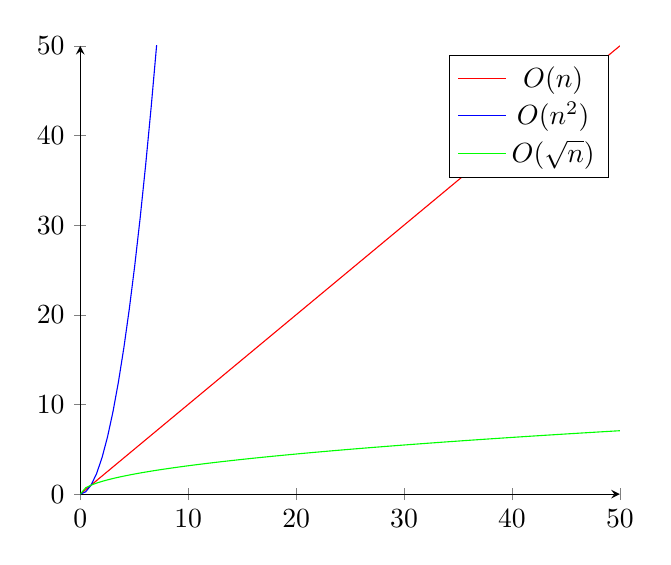
\begin{tikzpicture}
      \begin{axis}[ axis lines = left, ymin=0, ymax=50, xlabel = {}, ylabel =
        {}, ]
        \addplot [ domain=0:50, samples=100, color=red, ]{x};
        \addlegendentry{$O(n)$}
            
        \addplot [ domain=0:50, samples=100, color=blue, ]{x^2};
        \addlegendentry{$O(n^2)$}

        \addplot [ domain=0:50, samples=100, color=green, ]{sqrt(x)};
        \addlegendentry{$O(\sqrt{n})$}
      \end{axis}
    \end{tikzpicture}
  \end{center}
  \caption{The graph does a lot of stuff. The graph does a lot of stuff. The
    graph does a lot of stuff. The graph does a lot of stuff. The graph does a
    lot of stuff. The graph does a lot of stuff. The graph does a lot of stuff.}
\end{figure}

\noindent
A program that runs in $O(N)$ would be a function that inputs an integer $N$ and
outputs every number up to $N$. This runs in $O(N)$ time because it does $1+N$
operations which results in $O(n)$:

\begin{python}
  def linearTime(N): for number in range(N): print(number)
\end{python}
\noindent
Since the program runs in $O(N)$ time, increasing the input by a factor of $10$
would also increase the number of operations done by a factor of $10$. \newline
\\*
The second example is a program that runs in quadratic time, $O(N^{2})$. Compared
to the first example, this program will print every number up to $N$, $N$ times.

\begin{python}
  def quadraticTime(N): for number in range(N): for number in range(N):
  print(number)
\end{python}

\vspace{5mm}
\noindent
The third program describes $O(\sqrt{n})$. It is a simple program that sums all
numbers up to $\sqrt{N}$.

\begin{python}
  import math

  def sqrtTime(N): sum = 0 for number in range(math.isqrt(N)): sum += number
  print(sum)
\end{python}

\subsection{Deterministic vs. Probabilistic}
A deterministic test is a one-hundred percent definite test for primes, that
gives no false positives. It either returns true if the number being tested if
prime, or false if the number is not prime. \newline
\\*
Probabilistic tests differ from deterministic tests by having a stochastic,
random factor in them. They are not one-hundred percent definite and therefore
sometimes will give false positives/negatives.

An example of a probabilistic test for the number $p$ would be to test a random
number below $p$ and see if it divides $p$ evenly. This test would give a lot of
false positives, because even if $p$ is composite, not all numbers below it will
divide it. The accuracy of the test, i.e. the probability that it returns a
correct answer, is higher if there is an increased amount of unique factors,
$k$, tested.

\subsection{Algorithms}

\subsubsection{Brute-force} \label{brute} The brute force method tests all the
integers, $n$, between $2$ and $p-1$ and checks if $n$ satisfies $n \equiv 0
\Mod{p}$. If the condition is satisfied, $n$ would be a divisor of $p$ which
would make $p$ not a prime. However, if the loop completes without finding any
divisors to $p$, then $p$ is prime. The brute force algorithm is a definite
test, since it follows the definition of a prime; $p$ is prime if and only if
there are no divisors except for 1 and $p$ itself. The algorithm's time
complexity is $O(N)$, meaning it increases linearly. \newline

\begin{python}
  Insert code here
\end{python}

\subsubsection{Smart Brute-force}
The smart brute force is a variant of the brute force algorithm (\ref{brute}).
By utilizing some properties of primes, the smart brute force has a time
complexity of $O(\sqrt{n})$ compared to the $O(N)$ complexity from the brute
force.

Since a prime can never have the factor $2$ in them, it is sufficient to
only test odd numbers (an if statement is written before to loop to test if it
has the factor $2$). On top of this, the smart brute force only
tests numbers up to and including $\sqrt{p}$. This is because, assuming that $p$
is composite, it must have at least 2 factors. If there exists a factor larger
than $\sqrt{p}$, it must have already been tested. This algorithm will run in
$O(\sqrt(n))$ time, which is much faster than the original brute force. \newline

\begin{python}
  Insert code here
\end{python}

\subsubsection{Lucas-Lehmer}
The Lucas-Lehmer algorithm is a deterministic primality test that only works for
Mersenne numbers. It takes advantage of a special property of Mersenne numbers:

\begin{mdframed}
  For some $p>2$, $M_p=2^p-1$ is prime if and only if $M_p$ divides $S_{p-2}$ where
  $S_0=4$ and $S_k=(S_{k-1})^2-2$ for $k>0$.
\end{mdframed}

There exists a proof for this, which will not be covered by this essay. \newline
\\*
The Lucas-Lehmer test has helped the GIMPS (Great Internet Mersenne Prime
Search) to find many of the largest primes known to man. This because the time
complexity of this test is much faster compared to the other tests. Another
advantage it has over some of the other tests, is that it is deterministic.

\subsubsection{Fermat}
The Fermat primality test \cite{algh:fermat} is a probabilistic algorithm that
resembles the Miller-Rabin test. The time complexity for the algorithm is $O(k
log^{2}n log log n log log log n)$. Although the long notation for the
algorithm, the speed of the test can be compared to Lucas-Lehmer.

Fermat's little theory \cite{fermat:little} states \textit{``If $p$ is prime and
  $a$ is not divisible by $p$ then: ''}

\begin{mdframed}
  \centering $a^{p - 1} \equiv 1 \Mod{p}$
\end{mdframed}

\subsubsection{Miller–Rabin}
The Miller-Rabin primality test \cite{algh:miller}, first discovered by Russian
mathematician M. M. Artjuhov in 1967, is an algorithm that has two versions. One
that is deterministic, and the other probabilistic. The deterministic version is
conditional, meaning that it relies on an unproven theorem, in this case, the
extended Riemann hypothesis \cite{riemann}. However, the probabilistic version
is unconditional, meaning that it does not depend on an unproven theorem. This
makes the probabilistic version reliable. If the extended Riemann hypothesis
were to be disproved, the deterministic version would fall apart. The
probabilistic version is also faster for bigger $n$ compared to the
deterministic version. The probabilistic is therefore chosen for this study.
\newline
\\*
The Miller-Rabin primality test is considered to be one of the fastest
algorithms to verify if an $n$ is prime or not. The time complexity for the
probabilistic version is $O(k log^{3}(n))$, where $k$ is the amount of rounds
the algorithm will perform. \newline
\\*
insert how it works here
\end{document}
